% !TeX program = lualatex
% !BIB program = biber
% Lualatex is important to render Fira fonts; with pdflatex it's just the regular one
% ratio 16:9 -- https://tex.stackexchange.com/questions/14336/

% compile two versions, inspired by https://tex.stackexchange.com/a/1501
% use the script "compile-pdf.sh"
\newif\ifhandout
% if flags.tex does not exist, create an empty file to be able to compile in TeXstudio
\input{flags}

\ifhandout
	\documentclass[12pt,aspectratio=169,handout]{beamer}
\else
	\documentclass[12pt,aspectratio=169]{beamer}
\fi

% adjust for 16:9
% https://tex.stackexchange.com/questions/354022/modifying-the-margins-of-all-slides-in-beamer
\setbeamersize{text margin left=0.3cm,text margin right=1.0cm} 

%\usepackage{xcolor}

%%% better TOC
\usetheme[subsectionpage=progressbar]{metropolis}

% name in footer
\setbeamertemplate{frame numbering}{\insertframenumber ~ | Dr.\ Martin Tutek}

% blocks with background globally
\metroset{block=fill}

% adjust the background to be completely white
\setbeamercolor{background canvas}{bg=white}

% typeset mathematics on serif
\usefonttheme[onlymath]{serif}

% better bibliography using biber as backend
\usepackage[natbib=true,backend=biber,style=authoryear-icomp,maxbibnames=30,maxcitenames=2,uniquelist=false,giveninits=true,doi=false,url=false,dashed=false,isbn=false]{biblatex}
% shared bibliography
\addbibresource{../dl4nlp-bibliography.bib}
% disable "ibid" for repeated citations
\boolfalse{citetracker}

\definecolor{76abdf}{RGB}{118, 171, 223}

\setbeamercolor{frametitle}{bg=76abdf, fg=white}

\newcounter{saveenumi}
\newcommand{\seti}{\setcounter{saveenumi}{\value{enumi}}}
\newcommand{\conti}{\setcounter{enumi}{\value{saveenumi}}}

\resetcounteronoverlays{saveenumi}

\usepackage{xspace}
% Emojis
\usepackage{emoji}
% Figs
\usepackage{graphicx}
\graphicspath{ {./img/} }


% for derivatives, https://tex.stackexchange.com/a/412442
\usepackage{physics}

\usepackage{tikz}
\usetikzlibrary{matrix, positioning}
\usetikzlibrary{angles,quotes} % for angles
\usetikzlibrary{backgrounds} % background
\usetikzlibrary{decorations.pathreplacing} % curly braces
\usetikzlibrary{calligraphy}
\usetikzlibrary{calc} % for neural nets

% for plotting functions
\usepackage{pgfplots}
\usepgfplotslibrary{dateplot}

% sub-figures
\usepackage{caption}
\usepackage{subcaption}

% Checkmark, xmark
\usepackage{pifont}% http://ctan.org/pkg/pifont

% book tabs
\usepackage{booktabs}

% caption*
\usepackage{caption}


% show TOC at every section start
\AtBeginSection{
	\frame{
		\vspace{2em}
		\sectionpage
		\hspace*{2.2em}\begin{minipage}{10cm}
			\tableofcontents[currentsection]
		\end{minipage}
	}
}

% argmin, argmax
\usepackage{amssymb}% http://ctan.org/pkg/amssymb
\usepackage{amsmath}

\DeclareMathOperator*{\argmax}{arg\!\max}
\DeclareMathOperator*{\argmin}{arg\!\min}
% softmax
\DeclareMathOperator*{\softmax}{soft\!\max}
% RNN
\DeclareMathOperator*{\rnn}{RNN}
% RNN star
\DeclareMathOperator*{\rnnstar}{RNN^{*}}
% bi-RNN
\DeclareMathOperator*{\birnn}{biRNN}

% bold math
\usepackage{bm}

% for \mathclap
\usepackage{mathtools}

% algorithms
\usepackage[noend]{algpseudocode}


% for neurons and layers in tikz
\tikzset{
	neuron/.style={draw, rectangle, inner sep=2pt, minimum width=0.75cm, fill=blue!20},
	param/.style={draw, rectangle, inner sep=2pt, minimum width=0.75cm, fill=green!20},
	constant/.style={draw, rectangle, inner sep=2pt, minimum width=0.75cm, fill=black!15},
	state/.style={rectangle, inner sep=2pt, minimum width=0.75cm, fill=black!5},
}

% for strike-through text
\usepackage[normalem]{ulem}


\title{Deep Learning for Natural Language Processing}
\subtitle{Lecture 9 -- Text generation 3: Transformers}
\date{June 13, 2023}
\author{Dr.\ Martin Tutek}
\institute{Ubiquitous Knowledge Processing  \hfill 
\includegraphics[height=1.cm]{img/ukp_logo.png} \\
Department of Computer Science\\
Technical University of Darmstadt \hfill \href{https://www.informatik.tu-darmstadt.de/ukp/ukp_home/index.en.jsp}{\underline{UKP Web}}}
%\titlegraphic{\hfill }

\begin{document}

\maketitle

\begin{frame}{Recap}
	In the previous lecture we:
	\begin{itemize}
		\item Introduced the encoder-decoder architecture \& why we need it
		\item Defined the three broad classes of NLP problems
		\item Shown that RNNs have problems when modeling long dependencies
		\item Introduced the attention mechanism, its abstraction and design choices
	\end{itemize}
\end{frame}


\begin{frame}{Recap: Encoder-decoder with attention}
	\begin{center}
		\begin{figure}[h]
			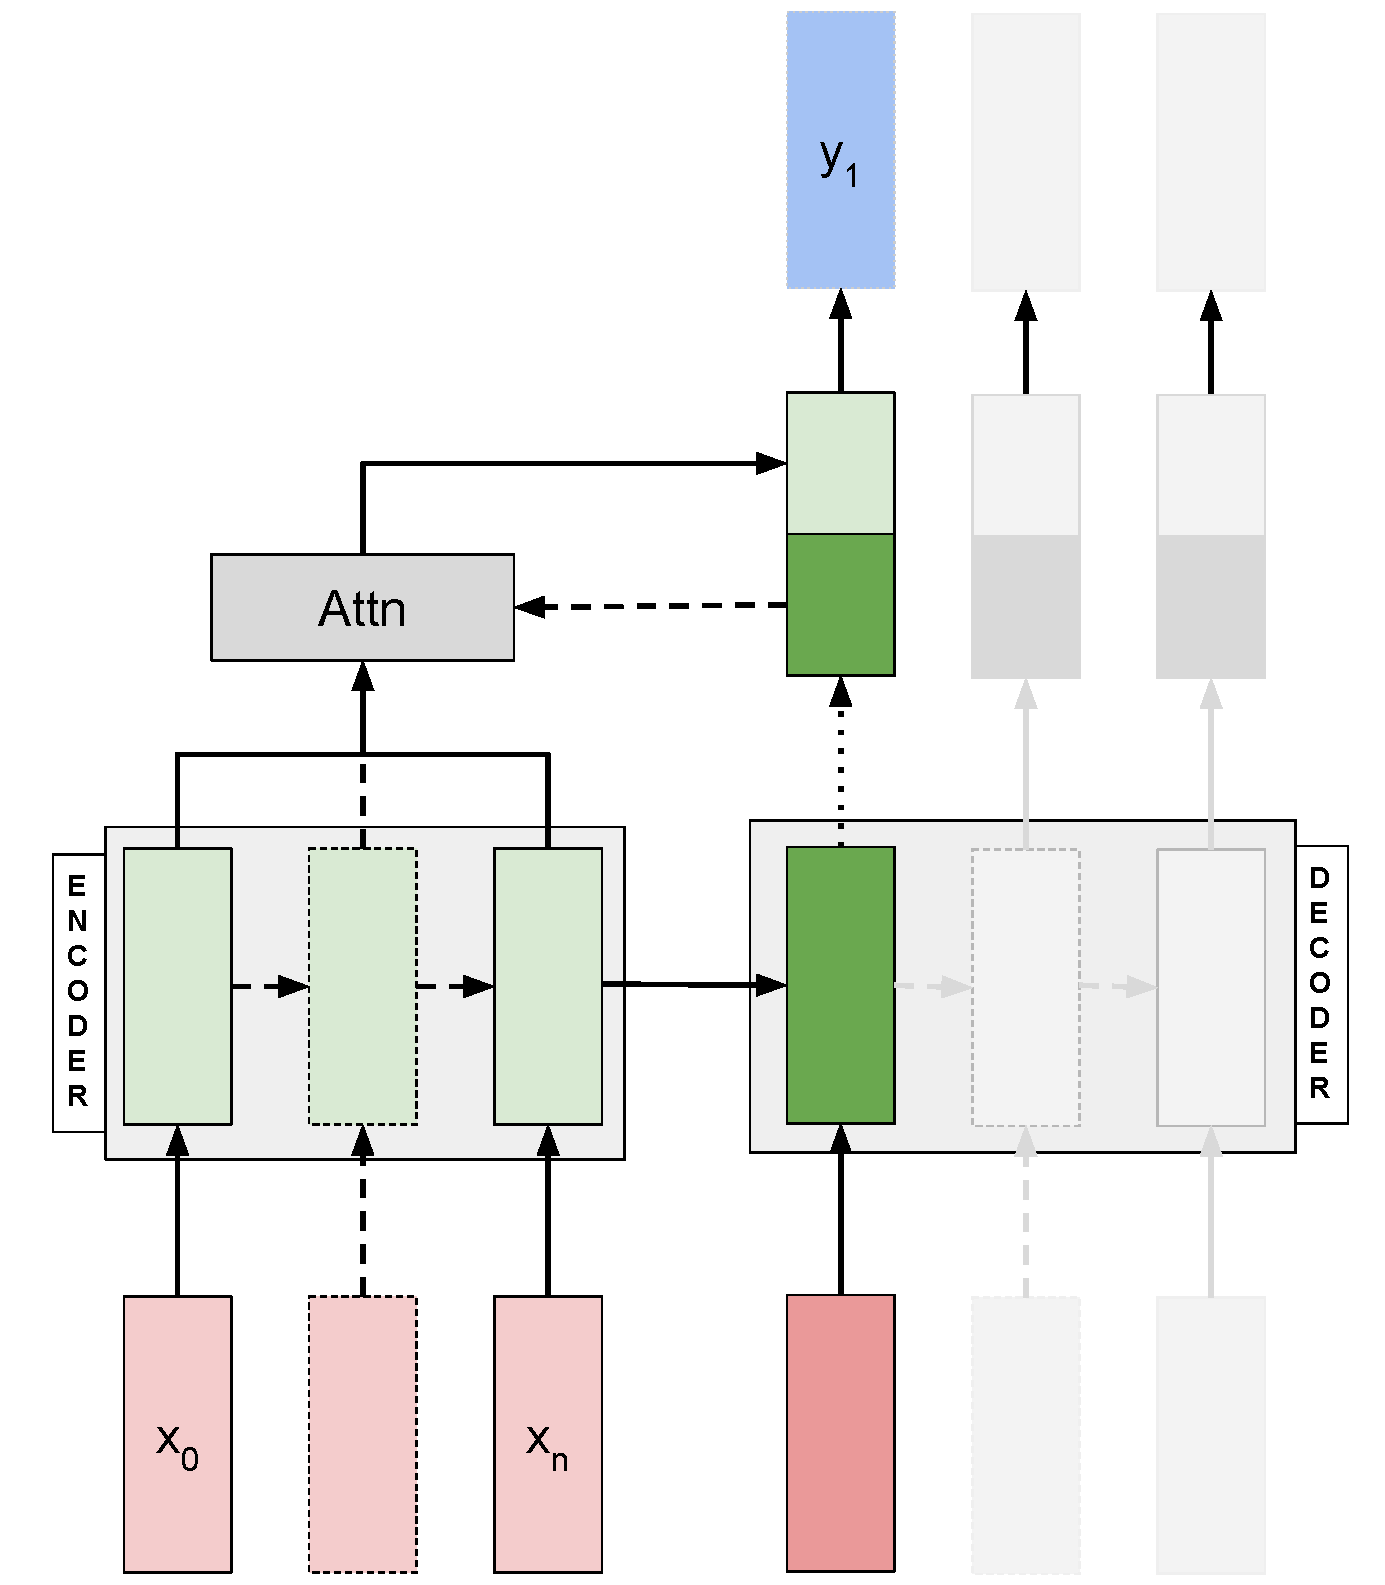
\includegraphics[height=7cm]{seq2seq_attn_encdec.pdf}
		\end{figure}
		\end{center}
\end{frame}


\begin{frame}{Motivation}

MLP -- fixed input sequence length 

RNN -- works well with \textbf{shorter} sequences

RNN + attention -- works well with both \textbf{shorter and longer} sequences

\pause

\begin{itemize}
	\item Why not use \textbf{only} attention?
\end{itemize}

\pause

\begin{center}
\begin{figure}[h]
	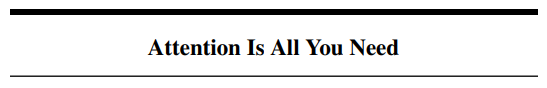
\includegraphics[height=2cm]{aiayn}
\end{figure}
\end{center}

\end{frame}

\begin{frame}{Prerequisites for attention-only networks}
	What do we \textbf{gain} from recurrent networks?
	\pause

	\begin{itemize}
		\item \textbf{Memory cells}: contain summaries of sequence read \textit{so far}
		\pause
		\begin{itemize}
			\item \textbf{However}, they have \textbf{limited} capacity -- we complement them with attention
		\end{itemize}
		\pause
		\item \textbf{Position} of a word in sequence
		\pause
		\begin{itemize}
			\item For each hidden state $s_{i}$, the current word embedding $x_i$ is added to the previous state $s_{i-1}$ -- the network can distinguish \textbf{word order}
			\pause
			\item \textbf{However}, it takes $n$ recurrence operations to process a sequence 
		\end{itemize}

	\end{itemize}
	\pause

	Do recurrent networks have any other \textbf{drawbacks}?

	\pause

	\begin{itemize}
		\item They \textbf{scale poorly} -- LSTMs are problematic to scale deeper than 4-8 layers
		\item \textbf{Closed vocabulary} -- so far, we assumed one word = one vector (no BPE)
	\end{itemize}
	\pause

	How to make attention-only networks work?

\end{frame}

\section{The Transformer}

\begin{frame}{The Transformer (\cite{Vaswani.et.al.2017})}
\begin{columns}[T] % align columns

	\begin{column}{.48\textwidth}

	\begin{figure}[h]
		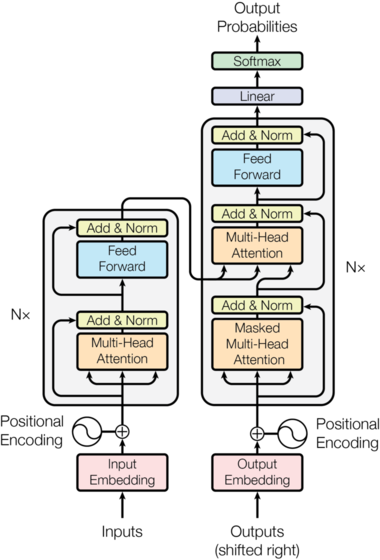
\includegraphics[height=7cm]{anno_transformer}
	\end{figure}
	\end{column}

	\begin{column}{.48\textwidth}
		What are the unknown elements?
		\pause
		\begin{itemize}
			\item \textbf{Multi-head} attention
			\item Add \& Norm
			\item \textbf{Positional} embeddings
			\pause
			\item \textbf{Open vocabulary} through BPE
		\end{itemize}	
	\end{column}

\end{columns}

\end{frame}

\subsection{Contextualized representations}

\begin{frame}{Contextualized representations}

Recall: \textbf{limitations} of word embeddings
\begin{block}{Polysemy, context independent representation}
	Some words have obvious multiple senses
	
	A \emph{bank} may refer to a financial institution or to the side of a river, a \emph{star} may an abstract shape, a celebrity, an astronomical entity
\end{block}
	
\pause

How do recurrent networks handle contextualization?

\pause
$$
s_i = f_{\text{rnn}} (s_{i-1}, x_i)
$$

\begin{itemize}
	\item Each state acts as a representation of the sequence \textbf{so far}
	\pause
\end{itemize}

\end{frame}

\begin{frame}{Contextualized representations}
	$$
	s_i = f_{\text{rnn}} (s_{i-1}, x_i)
	$$
	
	\begin{itemize}
		\item Each state acts as a representation of the sequence \textbf{so far}
		\pause
		\begin{itemize}
			\item Recall: \textbf{bidirectional} RNNs (left- and right-hand context)
			\item A state contains \textbf{cues} about the meaning of the current word \textbf{in context}
			\pause
		\end{itemize}
		\vspace{1em}
		\item \textbf{However}, the state has to act as both
		\begin{enumerate}
			\item A summary of the entire sequence
			\item The meaning of the current word in context
		\end{enumerate}
	\end{itemize}

\end{frame}

\begin{frame}{Contextualized representations}

	\begin{columns}[T] % align columns
	
		\begin{column}{.48\textwidth}
	
		\begin{figure}[h]
			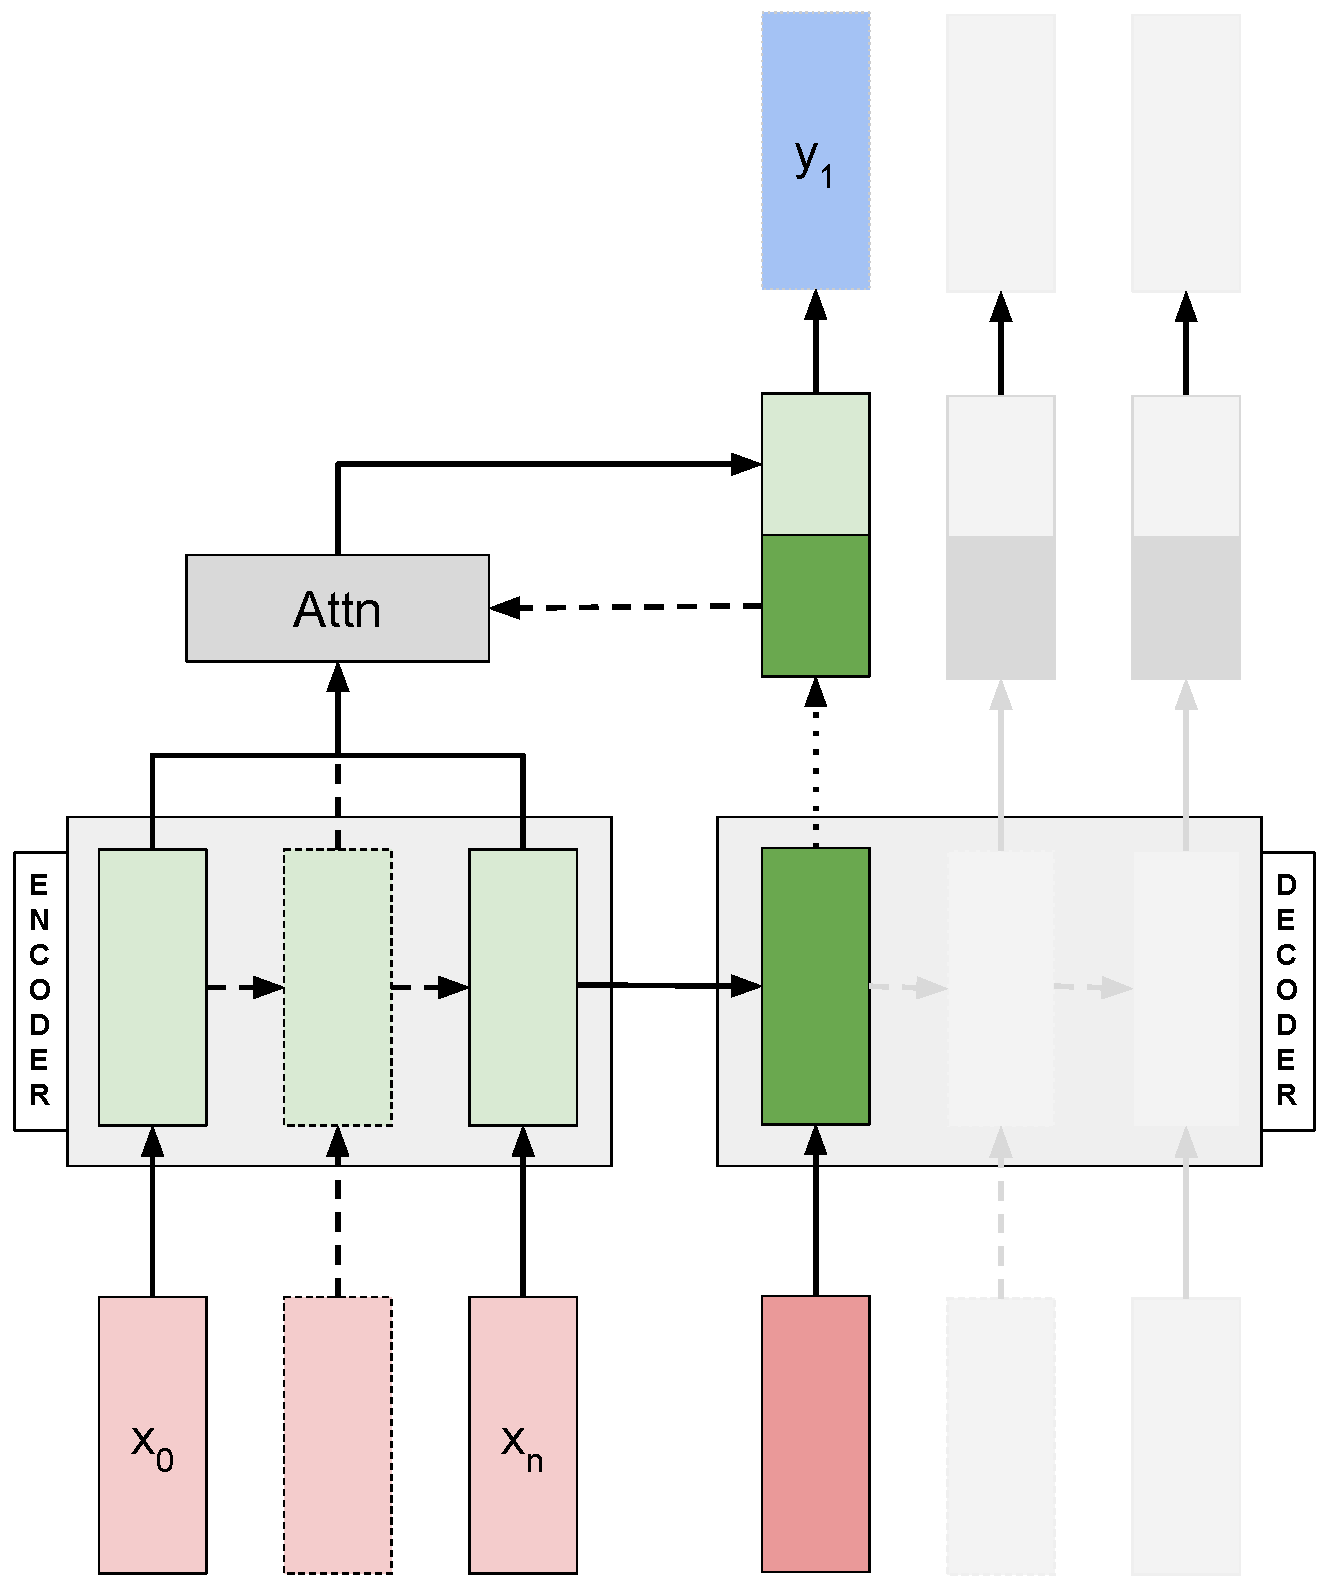
\includegraphics[height=7cm]{seq2seq_attention_t1.pdf}
		\end{figure}
		\end{column}
	
		\begin{column}{.48\textwidth}
			Step $1$ of encoder-decoder attention:
			\pause
			\begin{itemize}
				\item We obtain relevant information \textbf{for current state} from input sequence
				\pause
				\item This result of the attention operator should also contain \textbf{contextual cues}
			\end{itemize}
		\end{column}
	
	\end{columns}
	
\end{frame}


\begin{frame}{Contextualized representations}

	\begin{columns}[T] % align columns
	
		\begin{column}{.48\textwidth}
	
		\begin{figure}[h]
			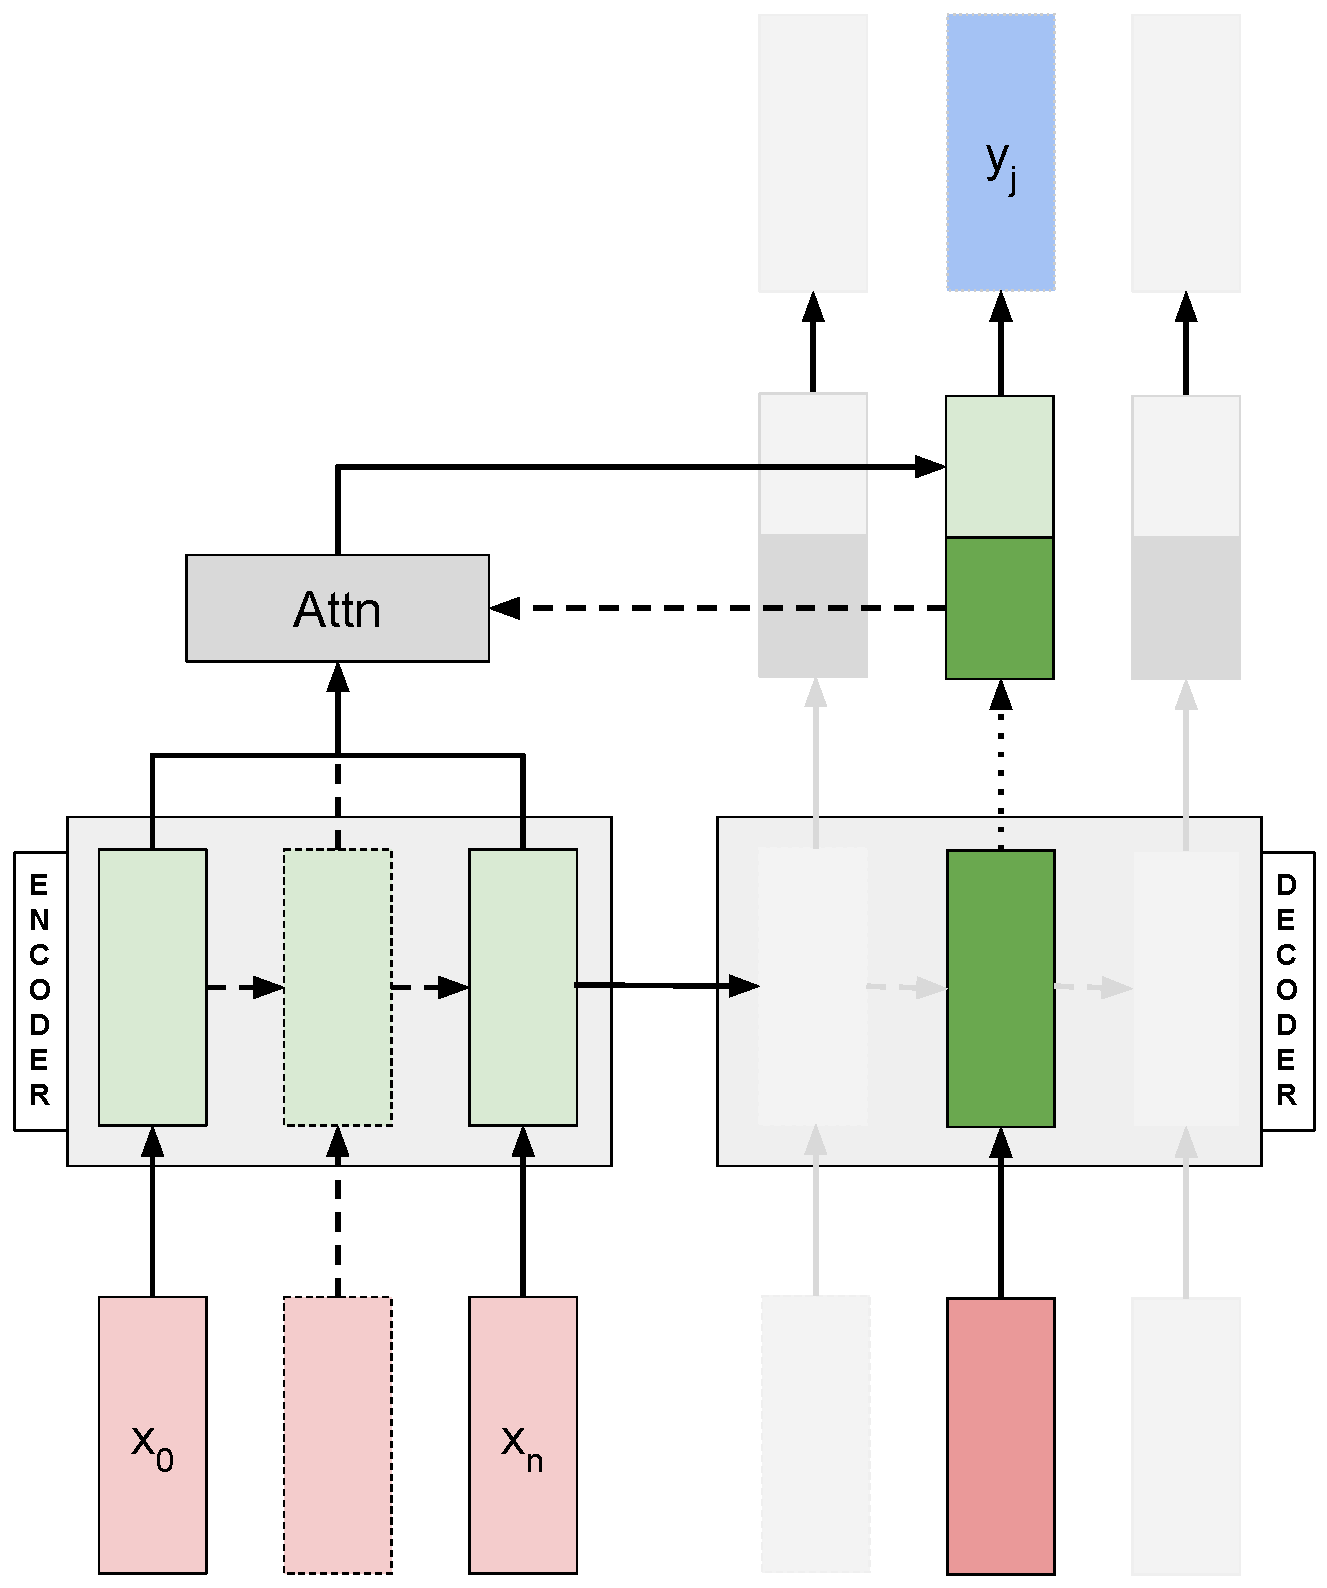
\includegraphics[height=7cm]{seq2seq_attention_t2.pdf}
		\end{figure}
		\end{column}
		\pause
		\begin{column}{.48\textwidth}
			\begin{figure}[h]
				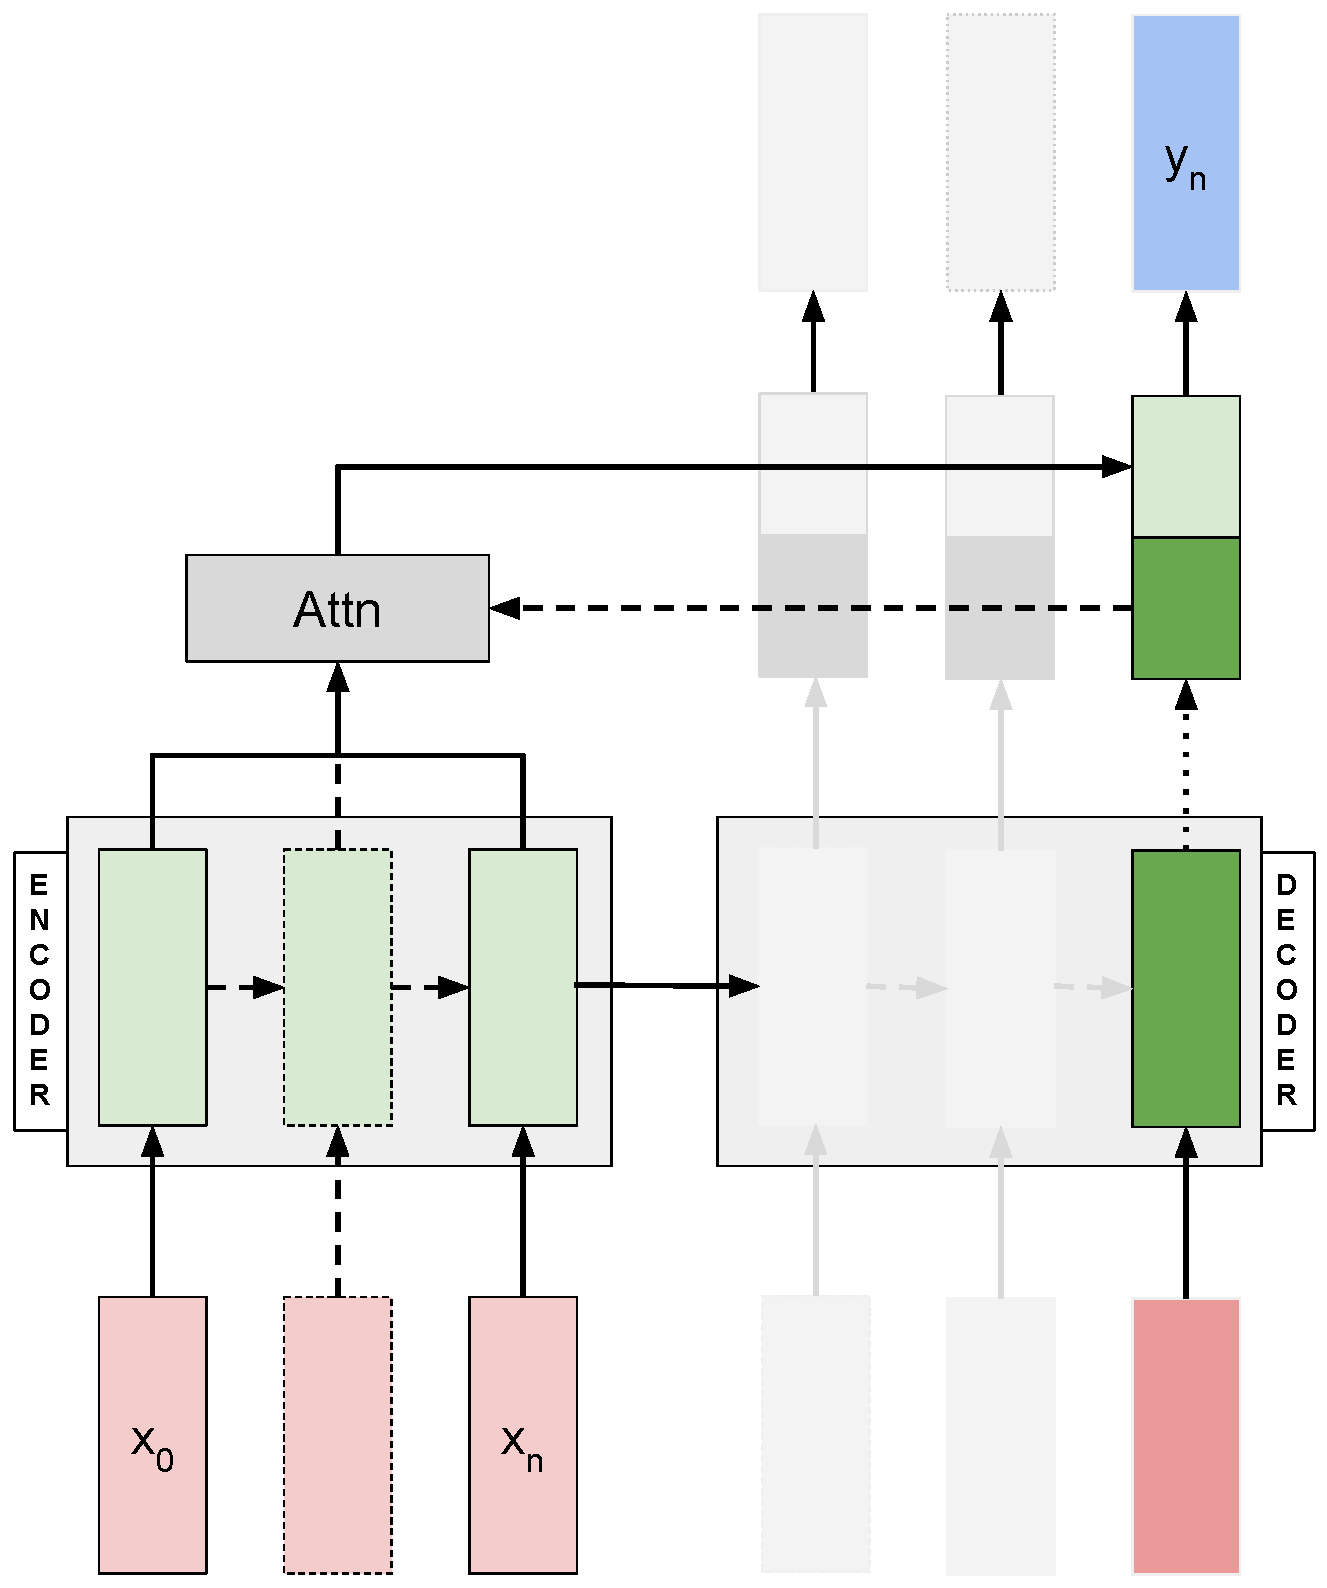
\includegraphics[height=7cm]{seq2seq_attention_t3.pdf}
			\end{figure}
		\end{column}
	
	\end{columns}
	
\end{frame}

\begin{frame}{Contextualized representations}
	Why not \textbf{cut out the middleman} (RNN)?
	\pause
	\begin{itemize}
		\item We use the RNN state as the \textbf{query} for attention
		\pause
		\item We could instead use the input \textbf{word representation}
	\end{itemize}
	\pause

	Recall: scaled dot-product attention

	\noindent\begin{minipage}{0.4\textwidth}
			$$
				a = \sum_i^n \alpha_i v_i
			$$ 
	\end{minipage}%
	\begin{minipage}{0.2\textwidth}
	\end{minipage}
	\begin{minipage}{0.4\textwidth}
			$$
				\hat{\alpha}_i = \frac{q^T \cdot k_i}{\sqrt{d_{\text{k} } } }
			$$
	\end{minipage}
	\pause

	Recall: what are the query, keys \& values (in encoder-decoder attention)?

	\noindent\begin{minipage}{0.29\textwidth}
		\vspace{1em}
		$$
			q = f_q(s^{\text{dec}}_t)
		$$ 
	\end{minipage}%
	\begin{minipage}{0.29\textwidth}
		$$
			K = f_k(\{s^{\text{enc}}_i\}_{i=1}^n)
		$$
	\end{minipage}
	\begin{minipage}{0.29\textwidth}
			$$
			 	V = f_v(\{s^{\text{enc}}_i\}_{i=1}^n)
			$$
	\end{minipage}

	\pause
	Where $f_q, f_k, f_v$ are arbitrary functions (neural network layers).

\end{frame}

\subsection{The Transformer attention block}

\begin{frame}{The Transformer attention block}

	\begin{columns}[T]
	\begin{column}{.48\textwidth}

		\begin{figure}[h]
			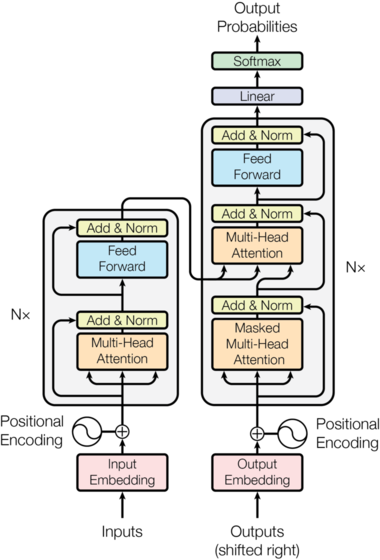
\includegraphics[height=7cm]{anno_transformer}
		\end{figure}
		\end{column}
		\begin{column}{.48\textwidth}
			\textbf{Encoder} part of the Transformer block

			\begin{itemize}
				\item Inputs: $\{\bm{x}^l_i\}_{i=1}^n; \quad \bm{x}_i \in \mathbb{R}^{d_m}$
				\item $x^0_i \to \text{word embeddings}$
				\pause 
			\end{itemize}

			Goal: \textbf{contextualize} word embeds.

			\begin{enumerate}
				\pause
				\item Transform \textbf{each} embedding to its query, key and value reprs.
				\pause
				\item Apply \textbf{pairwise} attention between all inputs 
				\pause
				\item Use the outputs as word embeddings for \textbf{next layer} 
			\end{enumerate}
		\end{column}
	\end{columns}
\end{frame}

\begin{frame}{The Transformer attention block}

	\begin{enumerate}
		\item Each layer $l$ has its own query, key and value linear transformation 
		$$
			\bm{W}^l_q, \bm{W}^l_k, \bm{W}^l_v \in \mathbb{R}^{d_m \times d_m}
		$$
		\pause
		\item Transform the inputs of the current layer $\{\bm{x}^l_i\}$ into the keys, queries and values
		$$
		\bm{Q} = \bm{W}_q (\{\bm{x}^l_i\}) \quad \bm{K} = \bm{W}_k (\{\bm{x}^l_i\}) \quad \bm{V} = \bm{W}_v (\{\bm{x}^l_i\})
		$$
		\pause
		\item Apply scaled dot-product attention
		$$
		\text{Attention} (\bm{Q},\bm{K},\bm{V}) = \text{softmax} \left( \frac{\bm{Q}\bm{K}^T}{\sqrt{d_m}}\right) \bm{V}
		$$

	\end{enumerate}


\end{frame}


\begin{frame}{The Transformer attention block: scaled dot-product}
	\begin{columns}[T] % align columns
	
		\begin{column}{.48\textwidth}
	
		\begin{figure}[h]
			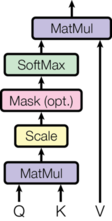
\includegraphics[height=5cm]{anno_transformer_attn_block}
			\caption*{Figure from \cite{Vaswani.et.al.2017}}
		\end{figure}
		\end{column}
	
		\begin{column}{.48\textwidth}
			$$
				\text{Attention} (\bm{Q},\bm{K},\bm{V}) = \text{softmax} \left( \frac{\bm{Q}\bm{K}^T}{\sqrt{d_m}} \right) \bm{V}
			$$
			\pause
			\begin{itemize}
				\item Matmul between $\bm{Q}$ and $\bm{K} \to$ \textbf{energy} 
				\pause
				\item Masking (why?)
				\begin{itemize}
					\item We might not want to attend to \textbf{all} tokens
				\end{itemize}
				\pause
				\item Output $=$ weighted sum
			\end{itemize}
		\end{column}
	
	\end{columns}
	
\end{frame}


\begin{frame}{The Transformer attention block: multi-head attention}

		\begin{columns}[T]
		\begin{column}{.48\textwidth}
	
			\begin{figure}[h]
				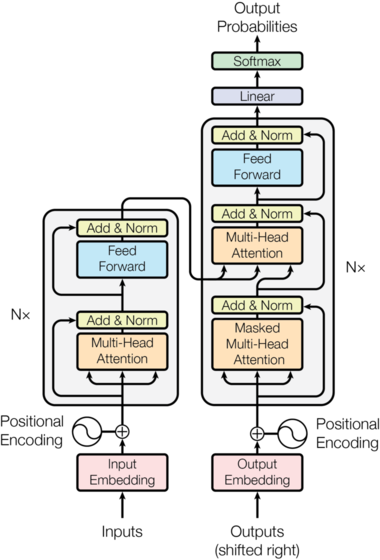
\includegraphics[height=7cm]{anno_transformer}
			\end{figure}
			\end{column}
			\begin{column}{.48\textwidth}
				However: we are using \textbf{multi-head} attention!
				\vspace{1em}
				\pause

				Idea: there could be \textbf{multiple aspects} in which two tokens can be similar
				\pause
				\begin{itemize}
					\item Intuition: \textit{each} hidden dimension $\approx$ one linguistic feature
					\item $\to$ perform \textbf{multiple} energy computations  
				\end{itemize}
			\end{column}
		\end{columns}
	\end{frame}


\begin{frame}{The Transformer attention block: multi-head attention}

	\textbf{Recall:} Transform the inputs of the current layer $\{\bm{x}^l_i\}$ into the keys, queries and values
	$$
	\bm{Q} = \bm{W}_q (\{\bm{x}^l_i\}) \quad \bm{K} = \bm{W}_k (\{\bm{x}^l_i\}) \quad \bm{V} = \bm{W}_v (\{\bm{x}^l_i\})
	$$

	\pause
	Each matrix $\bm{Q}, \bm{K}, \bm{V} \in \mathbb{R}^{n \times d_m}$, where $d_m$ is the \textit{model dimension}.

	\pause
	\textbf{Split} each query/key/value into $h$ \textbf{heads} (aspects) by \textit{reshaping}. 

	$$
		\bm{Q}, \bm{K}, \bm{V} \in \mathbb{R}^{n \times d_m} \to \bm{Q}, \bm{K}, \bm{V} \in \mathbb{R}^{n \times h \times d_m/h}
	$$
	\pause
	\begin{itemize}
		\item \textbf{Note}: $d_m$ \textbf{has} to be divisible by $h$
	\end{itemize}
	\pause 
	Remaining process continues as usual.

\end{frame}

\begin{frame}{The Transformer attention block: multi-head attention}

\textbf{Recall}: 3. Apply scaled dot-product attention
$$
	\text{Attention} (\bm{Q},\bm{K},\bm{V}) = \text{softmax} \left( \frac{\bm{Q}\bm{K}^T}{\sqrt{d_m}}\right) \bm{V} 
$$

\pause

Apply attention $h$ times \textbf{in parallel}, then \textbf{concatenate} the results.

\pause


$$
	\text{Attention}_j (\bm{Q}_j, \bm{K}_j, \bm{V}_j) = \text{softmax} \left( \frac{\bm{Q}_j \bm{K}_j^T}{ \sqrt{d_m / h} } \right) \bm{V}_j 
$$

\pause

Where $ \{ \bm{Q}, \bm{K}, \bm{V} \}^h_{j=1} $ are different \textit{heads}.

\end{frame}

\begin{frame}{The Transformer attention block: multi-head attention}

	\begin{columns}[T]
		\begin{column}{.48\textwidth}
	
			\begin{figure}[h]
				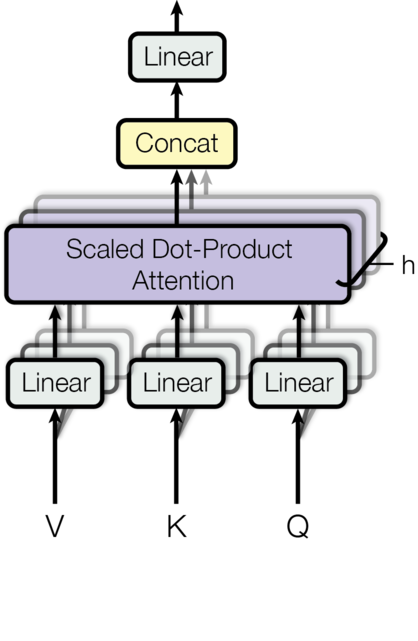
\includegraphics[height=7cm]{anno_trf_multihead}
			\end{figure}
			\end{column}
			\begin{column}{.48\textwidth}
				Although this entire process happens behind the scenes, we will still refer to (multi-head) attention as
				
				$$
					\text{Attention} (\bm{Q},\bm{K},\bm{V}) = \text{softmax} \left( \frac{\bm{Q}\bm{K}^T}{\sqrt{d_m}}\right) \bm{V} 
				$$

				for brevity.
			\end{column}
		\end{columns}

\end{frame}

\begin{frame}{The Transformer attention block: residual connection}

	\begin{columns}[T]
		\begin{column}{.48\textwidth}
	
			\begin{figure}[h]
				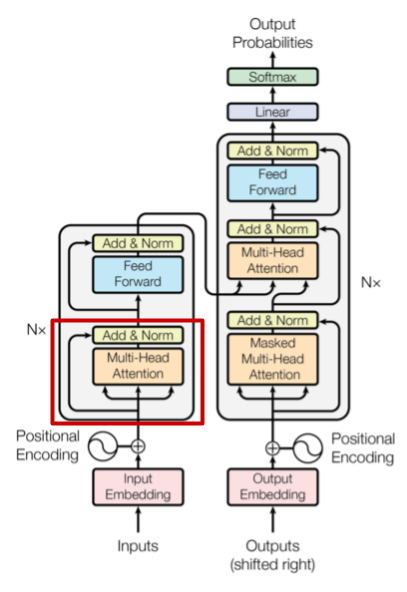
\includegraphics[height=7cm]{anno_trf_hlattn.png}
			\end{figure}
			\end{column}
			\begin{column}{.48\textwidth}
				We use \textit{residual connections} with the input of the layer
				\begin{enumerate}
					\item $\hat{x}^l$ is the output of attention
					$$ 
						\hat{x}^l = \text{Attention} (\bm{Q}^l,\bm{K}^l,\bm{V}^l)
					$$
					\item We apply the residual connection and normalize
					$$
						x^{l*} = \text{LayerNorm} ( x^l + \hat{x}^l )
					$$
					\seti
				\end{enumerate}
			\end{column}
		\end{columns}

\end{frame}

\begin{frame}{The Transformer attention block: position-wise linear layer}

	\begin{columns}[T]
		\begin{column}{.48\textwidth}
	
			\begin{figure}[h]
				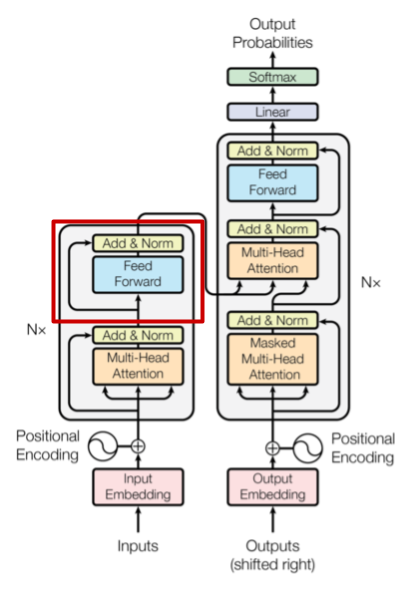
\includegraphics[height=7cm]{anno_trf_hllinear.png}
			\end{figure}
			\end{column}
			\begin{column}{.48\textwidth}
				\begin{enumerate}
					\conti
					\item We apply an extra \textbf{linear transformation} to each individual representation
				
					$$
						x^{l+1} = \text{LayerNorm} (x^{l*} + f^l_{hh} (x^{l*}))   
					$$

					Where $f_{hh}$ is an arbitrary transformation (single hidden layer NN)

					\item We use $x^{l+1}$ as the input to the \textbf{next} layer $l+1$
				\end{enumerate}
			\end{column}
		\end{columns}

\end{frame}

\subsection{Byte-pair encodings}

\begin{frame}{Byte-pair encodings}
	\textbf{Recall}: sub-word embeddings

	\begin{block}{Sub-word embeddings}
		Each character $n-$gram has its own embedding.

		Resolves the issues of \textbf{rare words}, \textbf{typos} and doesn't ignore the \textbf{morphology} of each word.

		However -- it scales poorly (there are \textbf{many} character $n-$grams)
	\end{block}

	\pause

	\textbf{Byte pair encodings} -- characters ($1$-grams / \textit{bytes}) can represent \textbf{any} word.


\end{frame}

\begin{frame}{Byte-pair encodings}

	\begin{block}{Byte-pair encodings}
		Start at \textbf{character} level. 
		
		Merge the two \textbf{most frequently co-occurring} characters into a \textbf{new character}. 
		
		Continue until you reach desired vocabulary size.
		\textbf{Each word} will always be represented.

	\end{block}

	\pause

	\textbf{Variants}: WordPiece, SentencePiece, subword-nmt (\href{https://github.com/google/sentencepiece}{\underline{GitHub}})

	\pause

	The differences are in the \textbf{merging criterion}:
	\pause
	\begin{itemize}
		\item \cite{Sennrich.et.al.2016.ACL} use \textbf{frequency} of co-occurrence;
		\item \cite{kudo2018subword} trains a \textbf{unigram language model}.
	\end{itemize}

\end{frame}

\subsection{Positional embeddings}

\begin{frame}{Positional embeddings}
	The Transformer processes all tokens \textbf{in parallel} -- there is \textbf{no information} about word order which in RNNs originated from recurrence. 

	\pause

	\textbf{Idea}: use functions which depend on \textbf{position of token in sequence}. The closer the tokens, the higher the similarity of the functions.
	
	\pause

	\begin{itemize}
		\item Sine and cosine waves
		$$
			PE_{(pos, 2i)} = \underbrace{\text{sin} ( \text{pos} / 10000^{2i / d_m})}_{\text{Even dimensions}}
		$$
		\pause
		$$
			PE_{(pos, 2i+1)} = \underbrace{\text{cos} ( \text{pos} / 10000^{2i / d_m})}_{\text{Even dimensions}}
		$$
		\pause
		\item We \textbf{sum} the positional embedding vector to the token embedding
	\end{itemize}

\end{frame}

\begin{frame}{Positional embeddings}
	\begin{center}
		\begin{figure}[h]
			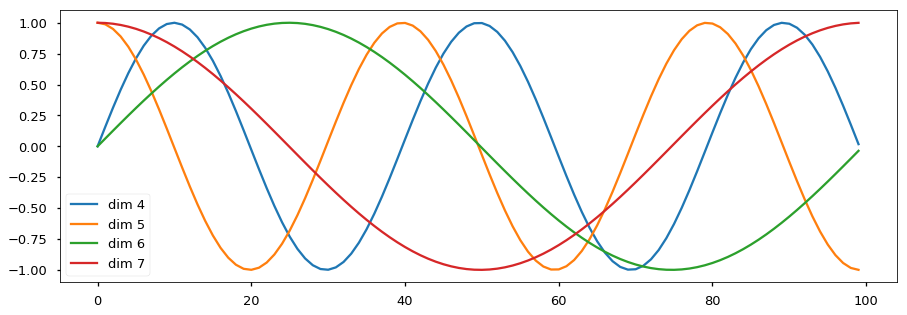
\includegraphics[height=5cm]{positional_embs}
		\end{figure}
		\end{center}
\end{frame}


\begin{frame}{Positional embeddings}
	Alternative: \textbf{trained} positional embeddings

	\pause
	\begin{itemize}
		\item Similar to word embeddings (byte pair embeddings)
		\item We randomly initialize a \textbf{position embedding matrix} and train it along with our model
		\pause
		\begin{itemize}
			\item \underline{Issues}?
			\pause
			\item How \textbf{large} is this position embedding matrix?
			\item What if test data contains sequences \textbf{longer} than training data? 
		\end{itemize}
	\end{itemize}

\end{frame}


\section*{Recap}

% **Content**
%
%* Vanilla RNNs (and maybe vanishing/exploding gradient?)
%* LSTM cells
%* Bi-Directional LSTMs
%* Domain adaptation and multi-task learning (?) 
%
%**Notes**
%
%efficiency, bidirectionality, multi-layer RNNs, how to apply to different tasks, how to ensure no data leakage
%connection to LMs (using RNNs)?
%
%* Domain adaptation and multi-task learning (?) - should be somewhere early too

\begin{frame}{Takeaways}
	
\begin{itemize}
	\item Transformer networks are \textbf{fully attentional networks}
	\begin{itemize}
		\item More efficient than RNNs (process tokens in parallel)
		\item Scale better than RNNs (deeper networks)
	\end{itemize}
	\item Multi-head attention
	\begin{itemize}
		\item Split each token representation into $h$ parts, perform $h$ attention operations in parallel
		\item Increased expressivity
	\end{itemize}
	
	\item They require \textbf{positional embeddings}
	\begin{itemize}
		\item Parallel processing $=$ no information about word position
	\end{itemize}
	\item Byte pair encoding allows for \textbf{open vocabulary}
\end{itemize}
	
\end{frame}



\begin{frame}{License and credits}

	\begin{columns}
		\begin{column}{0.7\textwidth}
			Licensed under Creative Commons Attribution-ShareAlike 4.0 International (CC BY-SA 4.0)
		\end{column}
		\begin{column}{0.2\textwidth}
			
\includegraphics[width=0.9\linewidth]{img/cc-by-sa-icon.pdf}
		\end{column}
	\end{columns}
	
	\bigskip
	
	Credits
	
	\begin{scriptsize}
		
		Martin Tutek
		
		Content from ACL Anthology papers licensed under CC-BY \url{https://www.aclweb.org/anthology}
		
	
	\end{scriptsize}
	
\end{frame}



\end{document}

